\subsection{Исследование неподвижных точек}
\begin{definition}
        Неподвижной точкой системы $x = f(x)$ называется точка $x^*$ такая, что $f(x^*) = 0$.
\end{definition}
Для рассматриваемой в рамках задачи системы (\ref{eq:main_system}) это определение эквивалентно тому, что
$$
        \left\{
        \begin{aligned}
                & x_2^* = 0 \\
                & u - x_1^* - 3 \sin(3(x_1^*)^3) - x_1^* x_2^* = 0.
        \end{aligned}
        \right.
$$
Покажем, что данная система имеет единственное решение. Рассмотрим производную второго уравнения системы $g(x_1) = u - x_1 -  3 \sin(3x_1^3)$ при условии, что $x_2^* = 0$ и $u = \mbox{const}$
$$
        g'(x_1) = - 1 - 27\cos(3x_1^3)x_1^2 < 0,
$$
то есть функция $g(x_1)$ монотонно убывает. Заметим также, что $\lim_{x_1\to-\infty}g(x_1) = +\infty$ и $\lim_{x_1\to+\infty}g(x_1) = -\infty$, то есть функция $g(x_1)$ имеет ровно один корень.

Рассмотрим системы, дающие оптимальные траектории
\begin{equation}\label{eq:optimal_traectories}
        \left\{
        \begin{aligned}
                & x_2^* = 0 \\
                & \pm \alpha - x_1^* - 3 \sin(3(x_1^*)^3) = 0.
        \end{aligned}
        \right.
\end{equation}
Стоит отметить, что если точка $(x_1^*, 0)$ является решением одной системы, то точка $(-x_1^*, 0)$ будет решением для второй системы. В точке $(x_1^*, 0)$ происходит переключение, так как она лежит на прямой $x_2 = 0$.
\begin{figure}[h]
        \centering
        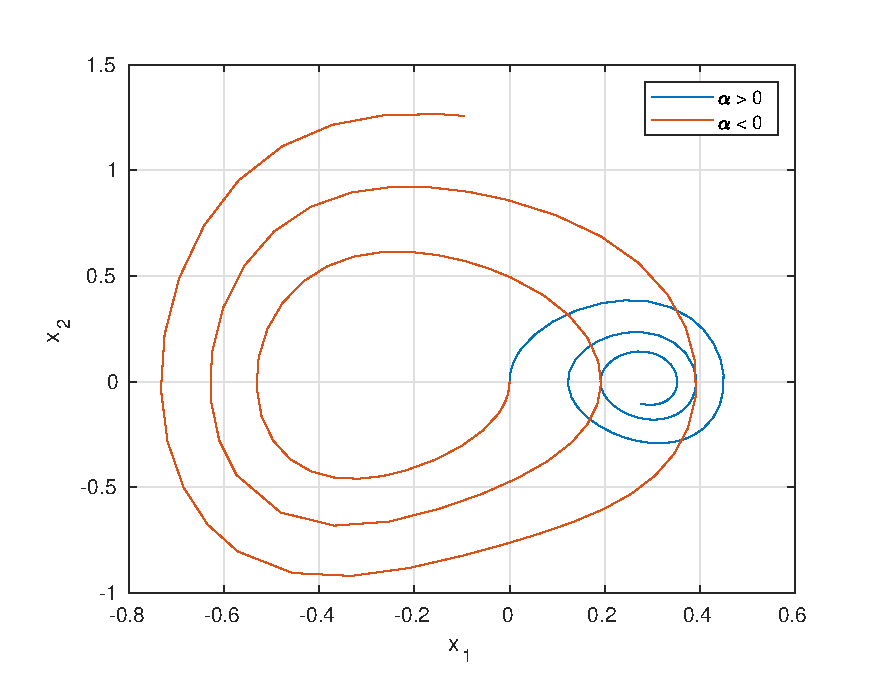
\includegraphics[width=0.49\linewidth]{research_of_the_system/fixed_points/a0-5t10.eps}
        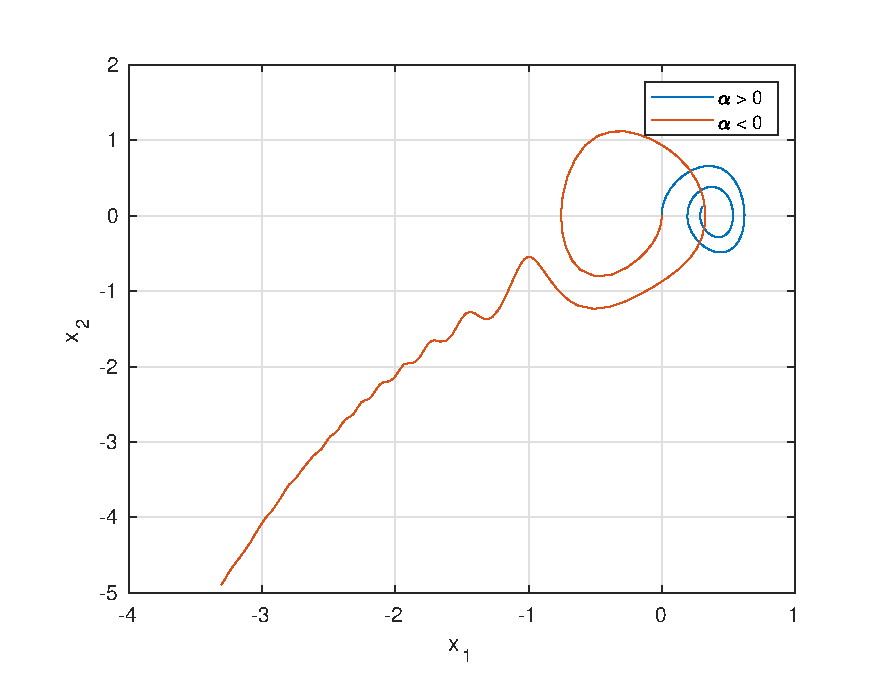
\includegraphics[width=0.49\linewidth]{research_of_the_system/fixed_points/a1t6.eps}
        \caption{Примеры поведения системы (\ref{eq:optimal_traectories}) для различных параметров (слева $\alpha = \frac{1}{2}$, справа $\alpha = 1$).}
        \label{img:fixed_points}
\end{figure}

Из Рис.~\ref{img:fixed_points} видно, что при определенном подборе параметров точки, построенные с применением теоремы~\ref{th:pmp} могут образовывать \textit{петли}, лежащие внутри множества достижимости. Также часть траекторий могут быстро уйти в бесконечность. Эти особенности необходимо учесть при потроении алгоритма.

Осталось ответить на вопрос: требуется ли при реализации алгоритма в окрестности неподвижных точек проводить более точные рассчеты, чтобы избежать попадания нежелательных точек в построенное множество достижимости. Забегая вперед, можно привести следующие результаты: из Рис.~\ref{img:fixed_points_2} видно, что 
неподвижная точка системы с положительным параметром находится в \textit{зоне покрытия} системы с отрицательным параметром, и наоборот. Так что дополнительные проверки и увеличение точности алгоритма в данном случае не потребуется.

\begin{figure}[h]
        \centering
        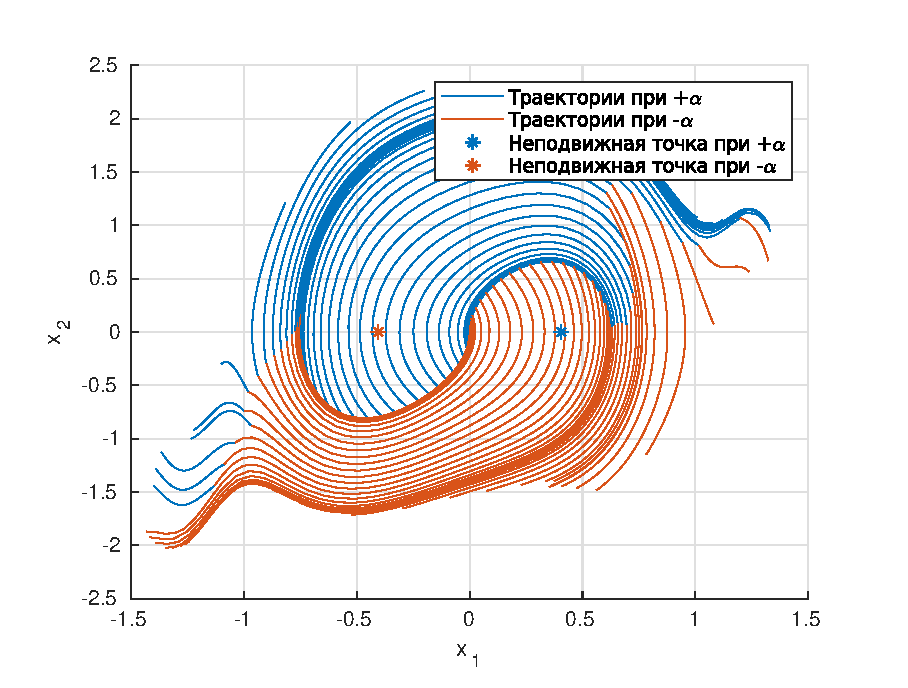
\includegraphics[width=0.49\linewidth]{research_of_the_system/fixed_points/a1t3.eps}
        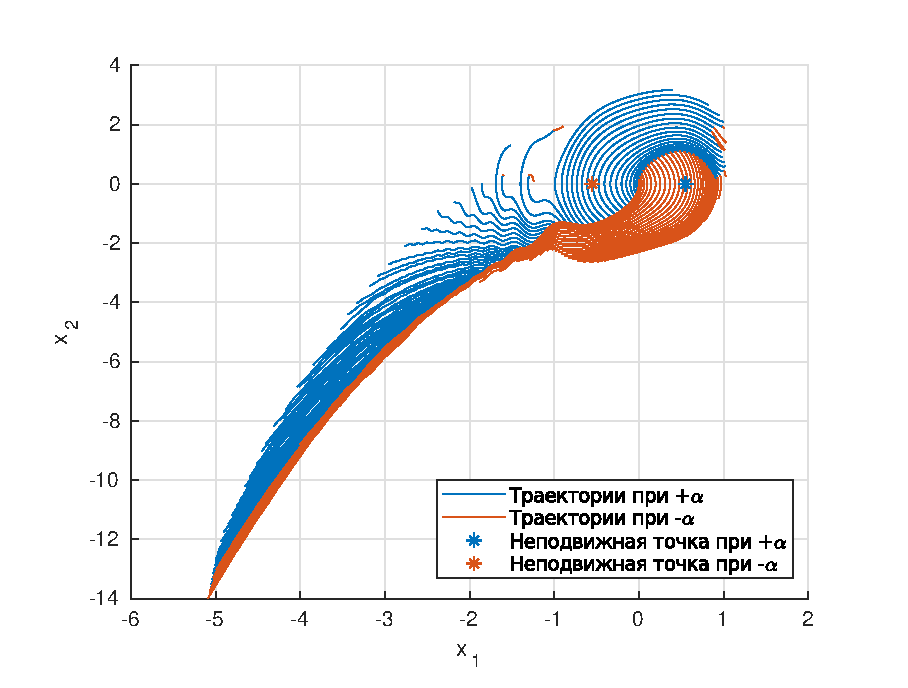
\includegraphics[width=0.49\linewidth]{research_of_the_system/fixed_points/a2t2.eps}
        \caption{Примеры поведения системы (\ref{eq:main_system}) для различных параметров (слева $\alpha = 1$, справа $\alpha = 2$).}
        \label{img:fixed_points_2}
\end{figure}